\documentclass[final,hyperref={pdfpagelabels=false}]{beamer}
\usepackage{grffile}
\mode<presentation>{\usetheme{VTCRINB}}
\usepackage[english]{babel}
\usepackage[latin1]{inputenc}
\usepackage{amsmath,amsthm, amssymb, latexsym}
\usepackage{fancyvrb}
\usepackage{framed}
%\usepackage{times}\usefonttheme{professionalfonts}  % obsolete
%\usefonttheme[onlymath]{serif}
\boldmath
%\usepackage[orientation=portrait,size=a0,scale=1.4,debug]{beamerposter}
\usepackage[orientation=portrait,size=a0,scale=1.05,debug]{beamerposter}
% change list indention level
% \setdefaultleftmargin{3em}{}{}{}{}{}


%\usepackage{snapshot} % will write a .dep file with all dependencies, allows for easy bundling

\usepackage{array,booktabs,tabularx}
\newcolumntype{Z}{>{\centering\arraybackslash}X} % centered tabularx columns
\newcommand{\pphantom}{\textcolor{ta3aluminium}} % phantom introduces a vertical space in p formatted table columns??!!

\listfiles

%%%%%%%%%%%%%%%%%%%%%%%%%%%%%%%%%%%%%%%%%%%%%%%%%%%%%%%%%%%%%%%%%%%%%%%%%%%%%%%%%%%%%%
\graphicspath{{figures/}}
 
\title{\vskip1ex\huge Bibliometric Analysis of Resting State Literature}
\author{Matthew K. Doherty$^1$, Ayesha Anwar$^1$, Sam Barberie$^1$, Caitlin Hinz$^1$, Michelle Kaplan$^1$, Anna Rachlin$^1$, \\ 
Michael P. Milham$^{1,2}$, Stephen M. LaConte$^{3,4}$ and R. Cameron Craddock$^4$}
\institute[1]{1 Child Mind Institute, New York, New York, \\
2 Nathan Kline Institute for Psychiatric Research, Orangeburg, New York \\
3 School of Biomedical Engineering and Sciences, Virginia Tech, Blacksburg, Virginia \\
4 Virginia Tech Carilion Research Institute, Roanoke, Virginia}
\posternum{\Large\vskip2ex 1-10-W}
\date[Sept. 5, 2012]{Sept. 5, 2012}

%%%%%%%%%%%%%%%%%%%%%%%%%%%%%%%%%%%%%%%%%%%%%%%%%%%%%%%%%%%%%%%%%%%%%%%%%%%%%%%%%%%%%%
\newlength{\columnheight}
\setlength{\columnheight}{101cm}

%%%%%%%%%%%%%%%%%%%%%%%%%%%%%%%%%%%%%%%%%%%%%%%%%%%%%%%%%%%%%%%%%%%%%%%%%%%%%%%%%%%%%%
\begin{document}
\begin{frame}
  \begin{columns}
    % ---------------------------------------------------------%
    % Set up a column 
    \begin{column}{.5\textwidth}
      \begin{beamercolorbox}[center,wd=\textwidth]{postercolumn}
        \begin{minipage}[T]{.96\textwidth}  % tweaks the width, makes a new \textwidth
          \parbox[t][\columnheight]{\textwidth}{ % must be some better way to set the the height, width and textwidth simultaneously
            % Since all columns are the same length, it is all nice and tidy.  You have to get the height empirically
            % ---------------------------------------------------------%
            % fill each column with content            
            \begin{block}{Introduction}
              \begin{itemize}
              \item Researchers are increasingly facing the challenges of searching, sorting, and digesting rapidly growing literatures within and across scientific disciplines.
              \item The Child Mind Institute (CMI) Librarian$^1$ initiative was created to address the growing need for comprehensive, hand-vetted reference libraries, tagged with descriptive labels capable of facilitating the rapid sorting and review of evolving literatures of interest.
              \item Mining of resting state (RS) literature is thus enabled by the CMI Librarian database. We performed a quantitative analysis of publication patterns within the resting state literature (a bibliometric analysis) to gain insight into
                \begin{itemize}
                \item trends of publication rates,
                \item prolific working groups of authors,
                \item experimental methods and areas of focus, and
                \item highest impact publications.
                \end{itemize}
              \end{itemize}              
            \end{block}
            \begin{block}{Publication Rates}
              \begin{itemize}
                  \item PubMed$^2$ queries were used to find growth of publication volume for resting state and all of fMRI. 
                  \item Piecewise exponential functions model growth of fMRI domain as well as its RS subdomain.
                   \end{itemize}
            \end{block}            
          \begin{block}{Working Group Analysis}
              \begin{itemize}
              \item Developed greedy algorithm using Dice coefficient-based heuristics to identify working groups $WG$.\\
              \begin{itemize}
			\item initialize $WG$ to $\emptyset$
			\item for each seed author $s$ in order of nonincreasing $|\text{pubs}(s)|$,
			\item \ \ set $a = s$
			\item \ \ do
			\item \ \ \ \ add $a$ to $A$
			\item \ \ \ \ find new author $a$ with $\arg \max_{a \notin A}(| \text{pubs}(a) \cap \text{pubs}(A)|)$
			\item \ \ loop until $|\text{pubs}(a)| < 10$ or $| \text{pubs}(a) \cap \text{pubs}(A)|/|\text{pubs}(A)| < 0.3$
			\item \ \ if $\sum | \text{pubs}(A_i) \cap \text{pubs}(A)| >= 50$ and $\sum I(|A \cap WG_i|/|WG_i| > 0.2) = 0$
			\item \ \ \ \ add $A$ to $WG$
		  \end{itemize}
              \end{itemize}
              \end{block}
            
            \begin{block}{Word Frequency Analysis}
                \begin{itemize}
                    \item Performed on n-grams from neuroimaging methods, cognitive ontology$^{3,4}$, and the PubBrain lexicon$^5$. 
                    	\item Term frequency (tf) was computed as the ratio of occurrences of each term to the number of words in the corpus. 
			\item Inverse document frequency (idf) was computed as $-\log (| \text{documents containing the term} |)$.
			\item Intuitively, high tf means the term is popular across the corpus, while high tf*idf means the term is popular in a small subset of the corpus.
			\item tf was plotted against tf*idf for the terms with the highest product of the two.
                \end{itemize}
            \end{block}
            \begin{block}{Citation Analysis}
                \begin{itemize}
                    \item Generated directed graph of citations directly from binary PDF publication files.
                    \begin{itemize}
                    	\item Performed fuzzy search for every possible publication title in each file using Python difflib.
				\item Resulted in graph of 1,196 publications (nodes) and 17,183 citations (edges).
                    \end{itemize}
                    \item Found publications with highest pagerank (impact estimate) using NetworkX$^6$ implementation.
                    \item Found mean and standard error of pageranks using jackknife procedure.
            	 \end{itemize}
            \end{block}
            \begin{block}{Results}
                \begin{center}
                \begin{columns}
              \begin{column}{.45\linewidth}
                  \begin{figure}
                      \begin{center}
                          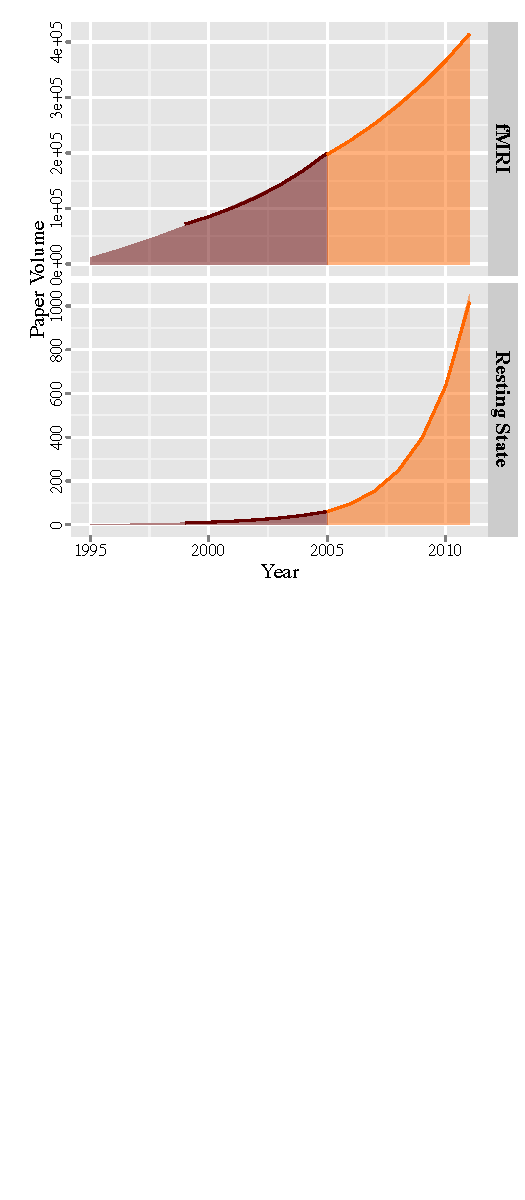
\includegraphics[width=.99\linewidth]{growth_rate.pdf}
                      \end{center}
                      \caption{\label{fig:growth_rate}Growth rates of fMRI and RSN volume}
                   \end{figure}
              \end{column}
              \begin{column}{.45\linewidth}
                  \begin{figure}
                      \begin{center}
                          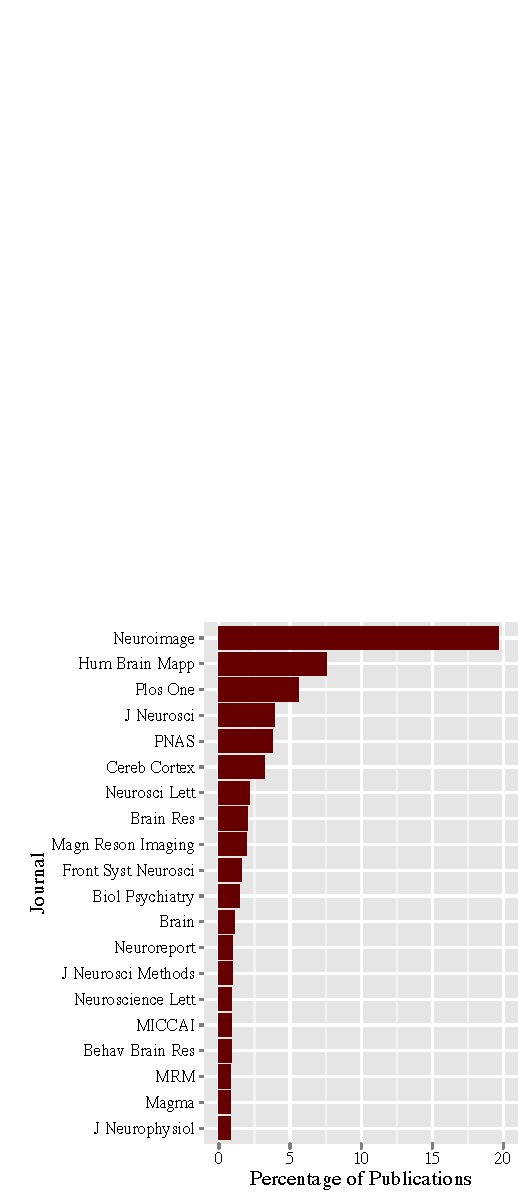
\includegraphics[width=.99\linewidth]{journal.pdf}
                      \end{center}
                      \caption{\label{fig:top_journals}Top journals by resting state publication count}
                   \end{figure}
              \end{column}
              \end{columns}
                \begin{itemize}
                \item Growth of RS literature is piecewise exponential with 33\% growth prior to 2005 and 47\% after. 
                \item In comparison, growth of fMRI literature was 29\% before 2005 and 18\% after.
                \item 27\% of RS literature was published in Neuroimage and HBM.
                \item 26\% of RS publications are open access, compared to 22\% in all of fMRI. 
                \end{itemize}     
\vskip1ex
\begin{itemize}
\item 23 authors (0.6\% of 3704 total) in 4 working groups cover 17.5\% of resting state publications. 
\item Mean papers by authors in these groups: 21.9. Overall mean: 0.310.
\item Mean papers in common between pairs of authors in same/different working groups: 10.7/0.11.
\item Working group authors (number publications in corpus by author):
\begin{itemize}
\item Milham, M P (41) and Kelly, A M (36) and Castellanos, F X (37) and Biswal, B (36)
\item Jiang, T Z (35) and Li, Kun-Cheng (27) and Yu, Chunshui (19) and Tian, Li-Xia (18) and Zhou, Yuan (15) and Liu, Yong (15) 
\item Gong, Qi-Yong (35) and Liu, Yi-Jun (21) and Liao, Wei (20) and Chen, Hua-fu (20) and Lu, Guang-Ming (18) and Zhang, Zhiqiang (17) and Zhong, Yuan (13) 
\item Schlaggar, Bradley L (19) and Petersen, Steven E (16) and Cohen, Alexander L (13) and Fair, Damien (13) and Dosenbach, Nico U F (10) and Miezin, Fran M (10)
\end{itemize}
\end{itemize}                   
              
              \end{center}
              \end{block}
              
            }
        \end{minipage}
      \end{beamercolorbox}
    \end{column}
    % ---------------------------------------------------------%
    % end the column

    % ---------------------------------------------------------%
    % Set up a column 
    \begin{column}{.5\textwidth}
      \begin{beamercolorbox}[center,wd=\textwidth]{postercolumn}
        \begin{minipage}[T]{.96\textwidth} % tweaks the width, makes a new \textwidth
          \parbox[t][\columnheight]{\textwidth}{ % must be some better way to set the the height, width and textwidth simultaneously
            % Since all columns are the same length, it is all nice and tidy.  You have to get the height empirically
            % ---------------------------------------------------------%
            % fill each column with content
            \begin{block}{Results (continued)}
                \begin{center}
                  \begin{figure}
                      \begin{center}
                          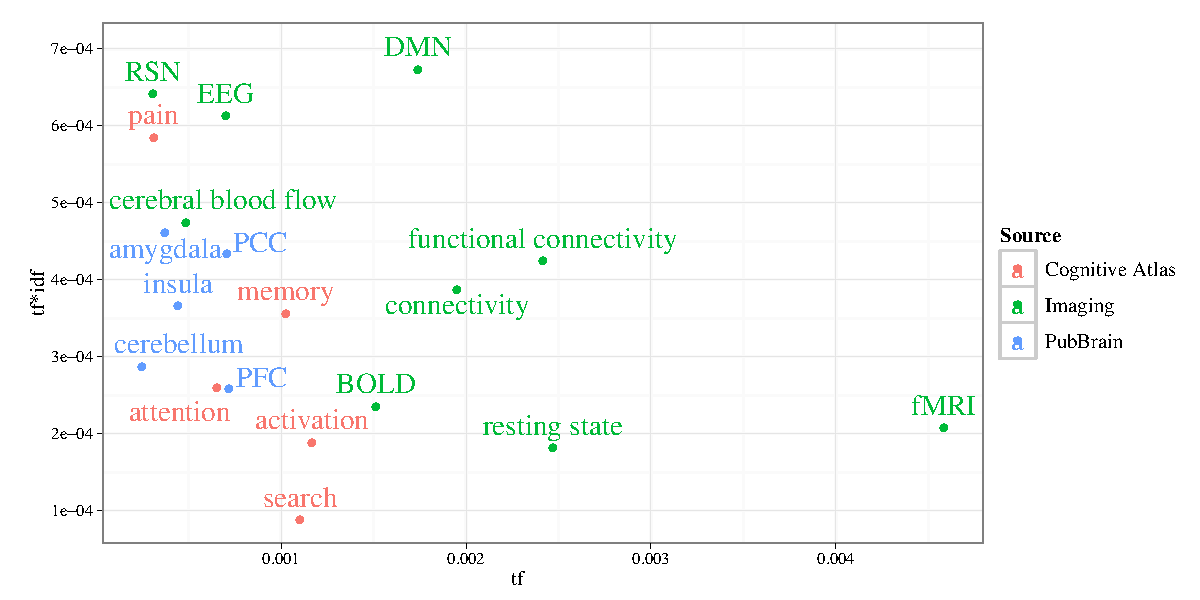
\includegraphics[width=.89\linewidth]{tfidf_100_v2.pdf}
                      \end{center}
                      \caption{\label{fig:citation_ranks}tf and tf*idf top terms}
                   \end{figure}
                \begin{itemize}
                \item The most frequent imaging modality is fMRI, which is the corpus domain.
                \item The most investigated cognitive domains are memory and activation. 
                \item The PFC, PCC, and insula are the most discussed brain regions.
                \end{itemize}
                  \begin{figure}
                      \begin{center}
                          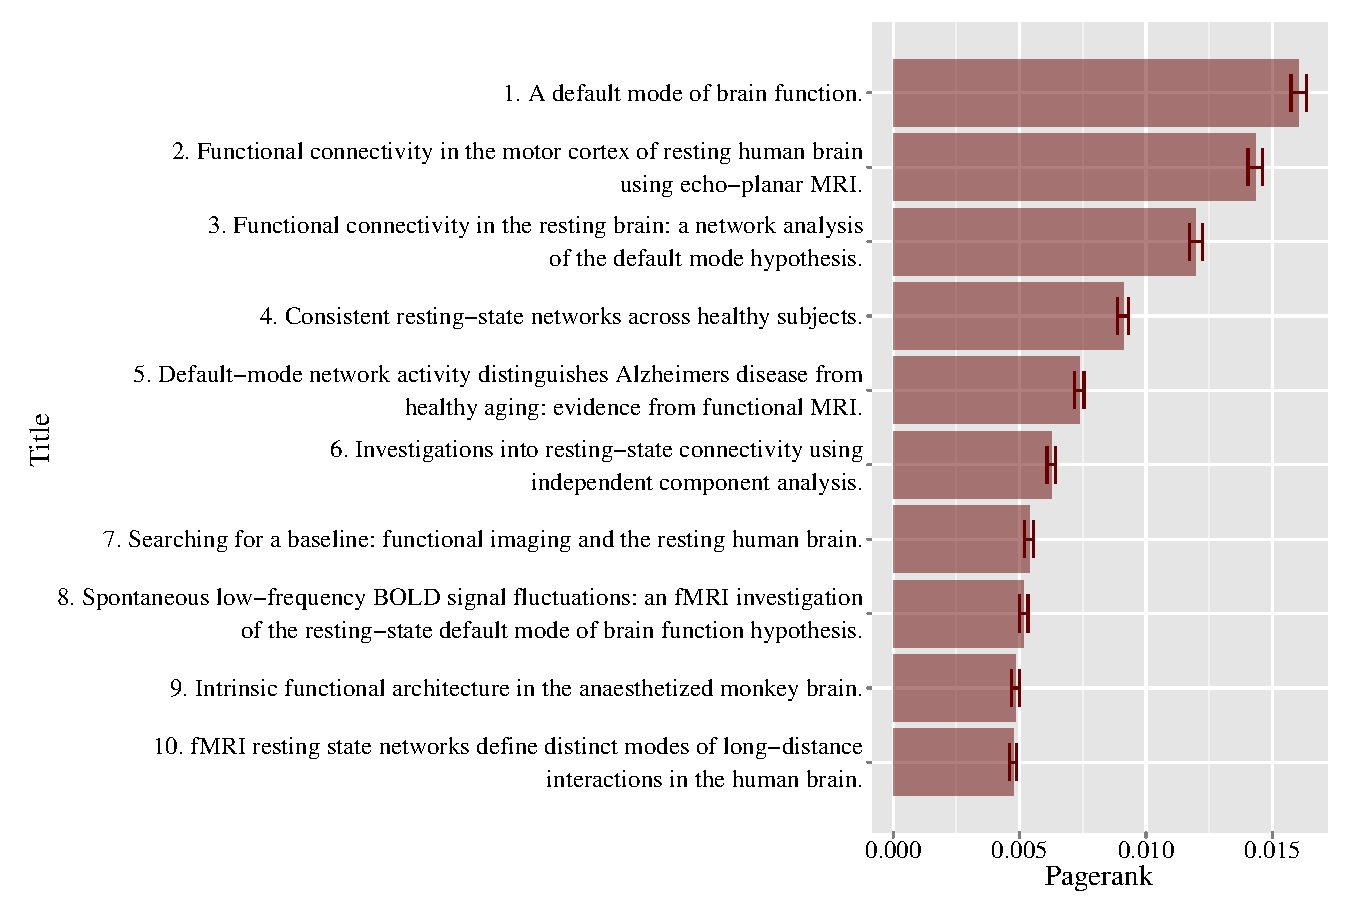
\includegraphics[width=.99\linewidth]{citations.pdf}
                      \end{center}
                      \caption{\label{fig:citation_ranks}Top resting state publications by pagerank}
                   \end{figure}
              \begin{columns}
              \begin{column}{.40\linewidth}
                              \vspace{0pt}
                \begin{center}
                \begin{itemize}
                	        \item The first few publications established the groundwork of the default  and resting state networks.	                  
                	        \item The top 10 publications are cited by 66\% of the corpus.      		
                		\item The top 1\% of publications account for 10\% of the total pagerank. 
			\item After these publications, page rank falls off more slowly, with the next 10\% of publications accounting for 40\% of the total pagerank. 
			\item Small world statistics: 
			\begin{itemize}
				\item Average clustering coefficient: 0.094
				\item Average path length: 4.4
			\end{itemize}				
                \end{itemize}
                \end{center}
              \end{column}              
              \begin{column}{.59\linewidth}
              \vspace{0pt}
                  \begin{figure}
                      \begin{center}
                          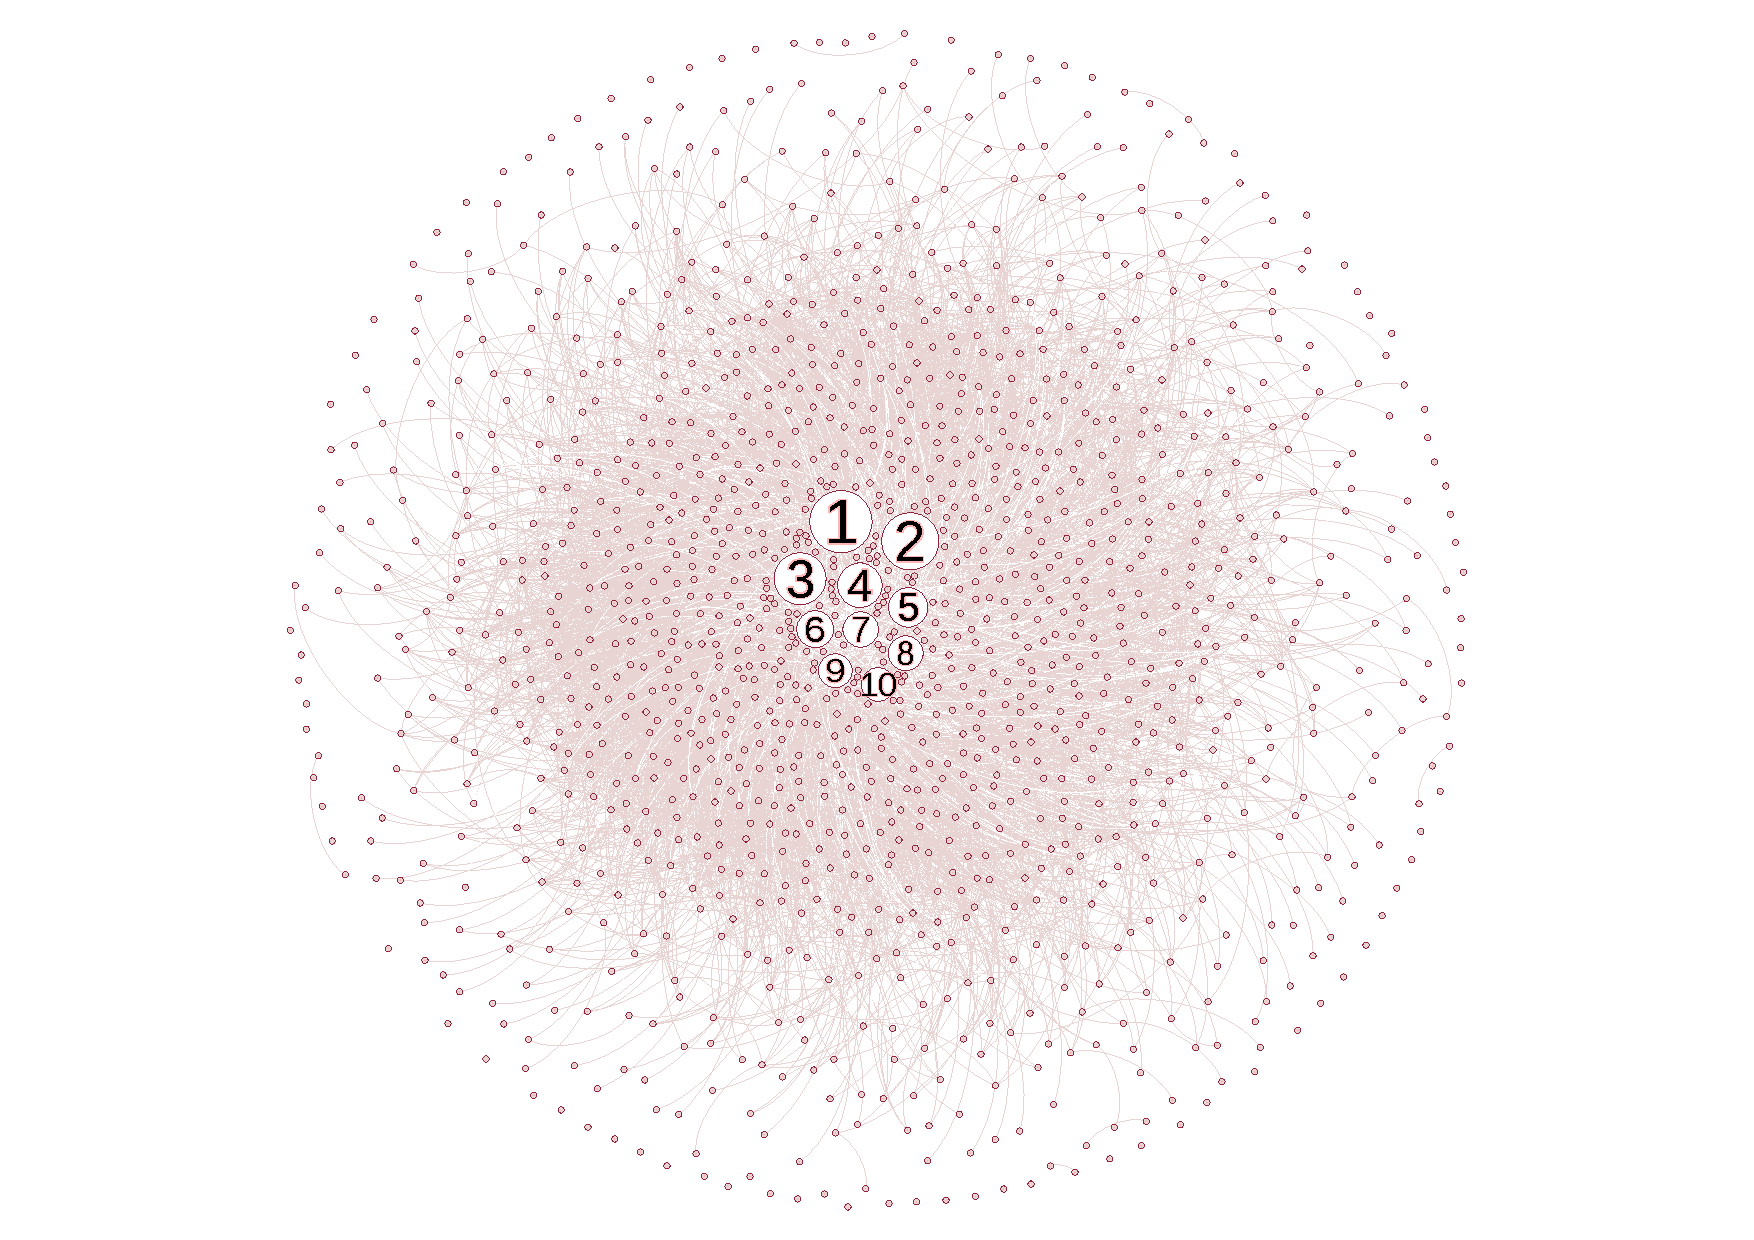
\includegraphics[width=.8\linewidth]{top_pagerank_graph2.pdf}
                      \end{center}
                      \caption{\label{fig:citation_graph}Top pageranked publications in complete graph}
                   \end{figure}       
              \end{column}
              \end{columns}
                   
            
                \end{center}

            \end{block}
            \begin{block}{Conclusions}
              \begin{itemize}
                  \item Bibliometric analysis lends valuable insight into the current state of the field, demonstrating its strength, areas of focus, and future potential. 
                  \item The growth of RS literature is currently faster than fMRI, the most common imaging modality in RS research. 
                  \item Analysis of open access showed that it is not universal in resting state or fMRI, but has a strong foothold.                   
                  \item A few prolific working groups together cover 17.5\% of RS publications, yet individually have little overlap.
                  \item The analysis identified a focus on PFC, involved with executive function, as well as the PCC, which is a central node of the DMN.  Activation was the most discussed cognitive domain, reflecting a current research trend. 
                  \item A handful of seminal publications provide much of the groundwork for the field. Relatively consistent pagerank among the remaining publications suggests that the field continues to grow in new and interesting directions.
                  \end{itemize}
            \end{block}
            %\begin{block}{References}
            %\end{block}
            \begin{block}{Acknowledgements}
            This research was supported by the Child Mind Institute Endeavor Scientist program.
            \end{block}
          }
          % ---------------------------------------------------------%
          % end the column
        \end{minipage}
      \end{beamercolorbox}
    \end{column}
    % ---------------------------------------------------------%
    % end the column
  \end{columns}
  %\vskip1ex
  \small\textcolor{black}{{\bf References:} 
$^1$Child Mind Institute. http://www.mendeley.com/profiles/cmi-librarian/ 2012,
$^2$National Center for Biotechnology Information, U.S. National Library of Medicine, http://www.ncbi.nlm.nih.gov/pubmed/ 2012,
$^3$Poldrack, R.A. http://www.russpoldrack.org/2011/07/my-analysis-of-ohbm-2011-abstracts.html 2011,
$^4$Poldrack, R.A., et. al. \textit{Front. Neuroinform.} 5(17) 2011,
$^5$Kalar, D. http://www.pubbrain.org/ 2012,
$^6$Hagberg, A.A., et. al. \textit{Proc. SciPy2008} 2008.\\
Top pageranked publications:
$^1$Raichle, M.E., et. al. \textit{Proc. Natl. Aca.d Sci.} 98(2) 2001,
$^2$Biswal, B., et. al. \textit{Magn. Reson. Med.} 34(4) 1995,
$^3$Greicius, M.D., et. al. \textit{Proc. Natl. Acad. Sci.} 100(1) 2003,
$^4$Damoiseaux, J.S., et. al. \textit{Proc. Natl. Acad. Sci.} 103(37) 2006,
$^5$Greicius, M.D., et. al. \textit{Proc. Natl. Acad. Sci.} 101(13) 2004,
$^6$Beckmann, C.F., et. al. \textit{Philos. Trans. R. Soc. Lond. B. Biol. Sci.} 360(1457) 2005,
$^7$Gusnard, D.A., et. al. \textit{Neuroscience} 2(10) 2001,
$^8$Biswal, B., et. al. \textit{Hum. Brain Mapp.} 26(1) 2005,
$^9$Vincent, J.L., et. al. \textit{Nature} 447(7140) 2007,
$^{10}$De Luca, M., et. al. \textit{Neuroimage} 29(4) 2005.
}

  %\tiny\hfill\textcolor{ta2gray}{Created with \LaTeX \texttt{beamerposter}  \url{http://www-i6.informatik.rwth-aachen.de/~dreuw/latexbeamerposter.php}}
  %\tiny\hfill{Created with \LaTeX \texttt{beamerposter}  \url{http://www-i6.informatik.rwth-aachen.de/~dreuw/latexbeamerposter.php} \hskip1em}
\end{frame}
\end{document}


%%%%%%%%%%%%%%%%%%%%%%%%%%%%%%%%%%%%%%%%%%%%%%%%%%%%%%%%%%%%%%%%%%%%%%%%%%%%%%%%%%%%%%%%%%%%%%%%%%%%
%%% Local Variables: 
%%% mode: latex
%%% TeX-PDF-mode: t
%%% End:
